\documentclass[12pt]{article}
\usepackage{amsfonts,amsthm,amsmath,amssymb,mathtools}
\usepackage{mathrsfs}
\usepackage{enumitem}
\usepackage{tikz-cd}
\usepackage{tikz}
\usepackage{geometry}
\usepackage{mlmodern}

\setlist[enumerate]{itemsep=-0.3em, topsep=0.3em}
\setlist[itemize]{itemsep=-0.3em, topsep=0.3em}

\geometry{letterpaper, portrait, margin=1in}

\setcounter{section}{0}
\setcounter{secnumdepth}{1}

\renewcommand{\thesection}{\S\arabic{section}}
\renewcommand{\thesubsection}{\arabic{subsection}}
% \newcommand{\dd}{\mathop{}\!\mathrm{d}}
\newcommand{\dd}{\mathop{}\!d}

\newtheorem{thm}{Theorem}
\newenvironment{theorem}[1]{
	\renewcommand{\thethm}{#1}
	\begin{thm}
		}{\end{thm}}

\newtheorem{lma}{Lemma}
\newenvironment{lemma}[1]{
	\renewcommand{\thelma}{#1}
	\begin{lma}
		}{\end{lma}}

\theoremstyle{definition}
\newtheorem{ex}{Exercise}
\newenvironment{exercise}[1]{
	\renewcommand{\theex}{#1}
	\begin{ex}
		}{\end{ex}}

\title{Differential Equations Cheat Sheet}
\date{}
\author{}

\begin{document}

\maketitle

\section{Basic Concepts}
\subsection{Definitions}
\begin{itemize}
	\item \textit{Order of a DE:} The highest-order derivative appearing in the DE
	\item \textit{Linear DE:} a DE in which there are no powers 2 of either the unknown function or its derivatives, and there are no products of the function or its derivatives with each other
	\item \textit{Initial Value Problem (IVP):} a differential equation that comes with one or more initial conditions for the unknown function and/or its derivatives
	\item \textit{Interval of Validity:} the largest possible interval on which a solution is valid and meets initial conditions
	\item \textit{General solution:} a solution which does not take into account initial conditions
	\item \textit{Actual solution:} a solution which takes into account initial conditions
	\item \textit{Explicit solution:} a solution which solves for the function in the form $y=y(x)$
	\item \textit{Implicit solution:} a solution which is not explicit
\end{itemize}

\subsection{Direction Fields}
What can you do with direction fields?
\begin{enumerate}
	\item Sketch solutions
	\item Determine long-term behavior
	\item Graph a family of solution/integral curves by starting with different initial values
\end{enumerate}

\subsection{Fundamental questions in Differential Equations}
\begin{enumerate}
	\item Does a solution exist?
	\item If a solution exists, is there a unique solution? What information do we need to narrow it down?
	\item If a solution exists, can we find it?
\end{enumerate}

\section{First Order Differential Equations}

\subsection{Linear Equations}
Form: \begin{equation*}
	y' + p(t)y = g(t)
\end{equation*}
where $p$ is continuous.
Solution process:
\begin{enumerate}
	\item Find a function $\mu(t)$ called an \textit{integrating factor} which satisfies $\mu(t)p(t)=\mu'(t)$.
	      \begin{enumerate}
		      \item Note that $p(t) = \frac{\mu'(t)}{\mu(t)} = (\ln(\mu(t)))'$.
		      \item Then $\mu(t) = e^{\int p(t) \dd t + k}$
		      \item Simplify by renaming $e^k$ to $k$: $\mu(t) = ke^{\int p(t) \dd t}$.
	      \end{enumerate}
	\item Multiply the DE by $\mu(t)$ to get $y'(t)\mu(t)+p(t)\mu(t)y(t) = g(t)\mu(t)$.
	\item Substitute $\mu'(t)$ to get $y'(t)\mu(t)+\mu'(t)y(t)=g(t)\mu(t)$.
	\item Use the product rule to get $(y(t)\mu(t))' = g(t)\mu(t)$.
	\item Integrate to get $y(t)\mu(t) + c = \int \mu(t)g(t) \dd t$.
	\item Algebra (and changing the sign of $c$) gives us the solution: \begin{equation*}
		      y(t) = \frac{\int\mu(t)g(t) \\d t + c}{\mu(t)}
	      \end{equation*}
\end{enumerate}

\subsection{Separable Equations}
Form: \begin{equation*}
	N(y) \frac{dy}{dx} = M(x).
\end{equation*}
Solve these by the shortcut (which can be made rigorous by substituting $u = y(x)$)\begin{equation*}
	\int N(y)dy = \int M(x)dx.
\end{equation*}
In general, this gives an implicit solution.

\subsection{Exact Equations}
Form:\begin{equation*}
	M(x, y) + N(x, y)\frac{dy}{dx}=0
\end{equation*}
where $M$ and $N$ are continuous and $M_y = N_x$.
Solution (after checking that the equation is exact by the condition above): \begin{equation*}
	\int M(x, y) dx - \int N(x, y) dy = c.
\end{equation*}
This solution is implicit and general.

\subsection{Bernoulli Differential Equations}
Form: \begin{equation*}
	y' + p(x)y = q(x)y^n
\end{equation*}
where $p$ and $q$ are continuous and $n \in \mathbb{R}$.
Solution process \begin{enumerate}
	\item Multiply by $y^{-n}$.
	\item Substitute $u = y^{1-n}$, so $u' = (1-n)y'y^{-n}$ and \begin{equation*}
		      \frac{1}{1-n}u' + p(x)u = q(x)
	      \end{equation*}
	\item Solve the linear equation above.
	\item Rewrite in terms of $y$.
\end{enumerate}

\subsection{More substitutions}
\begin{equation*}
	\begin{array}{l|l|l}
		\text{Form}                           & \text{Substitute}  & \text{Result}    \\
		\hline y' = F\left(\frac{y}{x}\right) & u(x) = \frac{y}{x} & \text{Separable} \\
		y' = G(ax+by)                         & u(x)=ax+by         & \text{Separable}
	\end{array}
\end{equation*}

\subsection{Existence Theorems}
\begin{enumerate}
	\item Given an IVP \begin{equation*}
		      y' + p(t)y = g(t), \hspace{1em} y(t_0) = y_0,
	      \end{equation*}
	      if $p(t)$ and $g(t)$ are continuous on an interval containing $t_0$, then there is a unique solution, and the interval of validity is the largest such interval.
	\item Given an IVP \begin{equation*}
		      y' = f(t, y), \hspace{1em} y(t_0) = y_0,
	      \end{equation*}
	      if $f(t, y)$ and $f_y$ are continuous in some rectangle $\alpha < t < \beta$, $\gamma < y < \delta$ containing $(t_0, y_0)$, there is a unique solution, and the interval of validity is \textit{contained in} $\alpha < t < \beta$.
\end{enumerate}

\subsection{Modeling with First Order DEs}
There are a few main types of situations we model with First Order ODEs: mixtures, population dynamics, and falling objects.

For mixtures, we have a tank of fluid with a substance dissolved in it, a substance entering the fluid, and a substance exiting the fluid.
Letting $Q(t)$ be the amount of the substance dissolved in the liquid, we use the ``equation'' \begin{align*}
	\text{Rate of change of $Q(t)$} & = \text{rate at which substance enters the tank} \\
	                                & - \text{rate at which substance exits the tank.}
\end{align*}

Similarly, for populations, we use \begin{align*}
	\text{Rate of change of $P(t)$} & = \text{rate at which population enters the region} \\
	                                & - \text{rate at which population exits the region.}
\end{align*}

For falling objects, use Newton's Second Law in the form \begin{equation*}
	mv' = F(t, v)
\end{equation*}
where $F$ includes gravity ($g = 9.8\,\text{m}/\text{s}^2$) and air resistance.
Choose your coordinate system well and stick with it.

\subsection{Equilibrium Solutions}
A realistic population growth model is the \textit{logistic growth equation}: \begin{equation*}
	P' = r\left(1 - \frac{P}{K}\right)P
\end{equation*}
where $r$ is called the \textit{intrinsic growth rate} and $K$ is the \textit{saturation level} or \textit{carrying capacity}.

\begin{figure}[h] \centering
	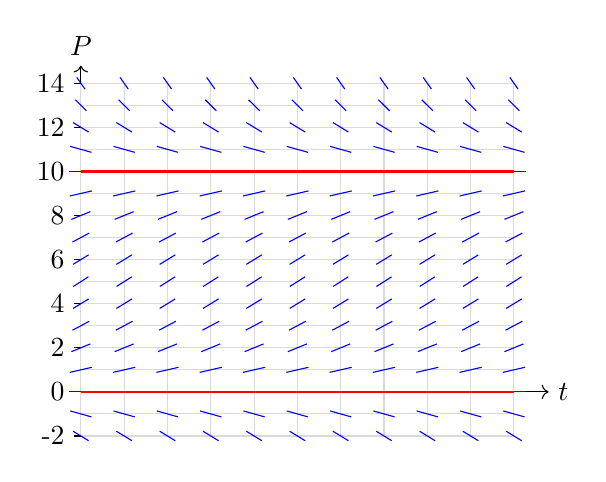
\begin{tikzpicture}[x=0.55cm,y=0.28cm] \draw[->] (0,0) -- (10.8,0) node[right] {$t$}; \draw[->] (0,-2) -- (0,14.8) node[above] {$P$}; \draw[gray!30, step=1] (0,-2) grid (10,14); \foreach \p in {-2,0,2,4,6,8,10,12,14} \draw (0,\p) -- (-0.15,\p) node[left] {\p}; \foreach \tval in {0,1,...,10} { \foreach \pval in {-2,-1,...,14} { \pgfmathsetmacro{\m}{0.5*(1-\pval/10)*\pval} \pgfmathsetmacro{\dx}{0.28/sqrt(1+\m*\m)} \pgfmathsetmacro{\dy}{0.28*\m/sqrt(1+\m*\m)} \draw[blue] ({\tval-\dx},{\pval-\dy}) -- ({\tval+\dx},{\pval+\dy}); } } \draw[red, thick] (0,0) -- (10,0); \draw[red, thick] (0,10) -- (10,10); \end{tikzpicture}
	\caption{Direction field for $P'=r\left(1-\frac{P}{K}\right)P$ where $r = 0.5$ and $K = 10$.}
\end{figure}

This is an example of an \textit{autonomous differential equation}, which is an equation of the form \begin{equation*}
	\frac{dy}{dt} = f(y).
\end{equation*}
For these, we call points where $\frac{dy}{dt} = 0$ \textit{equilibrium points} or \textit{equilibrium solutions}, and we can classify them into three types based on what happens to $y'$ in the regions of the graph which lie between them and other equilibrium solutions (or infinity): \begin{enumerate}
	\item \textit{Unstable}: nearby solutions tend away from the equilibrium point
	\item \textit{Asymptotically stable}: nearby solutions tend toward the equilibrium point from both sides
	\item \textit{Semi-stable}: nearby solutions tend toward the equilibrium point on one side and away from it on the other side.
\end{enumerate}

\subsection{Euler's Method}

We can approximate actual values of a solution to an IVP by starting with the initial value and then approximating, in steps, the ``next'' point using the tangent line, until we want to stop. This is called \textit{Euler's method}.

\section{Second Order Differential Equations}

\subsection{Basic Concepts}
Linear second order differential equation: \begin{equation*}
	p(t)y'' + q(t)y' + r(t)y = g(t).
\end{equation*}
Most of the time, the coefficients will be constant (non-constant is much harder): \begin{equation*}
	ay'' + by' + cy = g(t).
\end{equation*}
The DE is \textit{homogeneous} when $g(t) = 0$ and \textit{nonhomogeneous} when $g(t) \neq 0$.

Principle of Superposition: if $y_1(t)$ and $y_2(t)$ are two solutions to a linear, homogeneous differential equation then so is \begin{equation*}
	y(t) = c_1y_1(t) + c_2y_2(t).
\end{equation*}

When there are two constants in the general solution, we generally need two initial conditions to determine an actual solution.

\subsection{Constant-coefficient, homogeneous, linear, second-order DEs}

Given a constant-coefficient, homogeneous, linear, second-order DE \begin{equation*}
	ay'' + by' + cy=0,
\end{equation*}
the \textit{characteristic equation} is \begin{equation*}
	ar^2 + br + c = 0.
\end{equation*}
If $r_1$ and $r_2$ are the two roots of the characteristic equation, then two solutions to the DE are \begin{align*}
	y_1(t) & = e^{r_1t} \\
	y_2(t) & = e^{r_2t}
\end{align*}
There are three types of roots: real and distinct, complex and distinct, and repeated roots. \begin{itemize}
	\item If $r_1$ and $r_2$ are both real and distinct, the general solution is \begin{equation*}
		      y(t) = c_1e^{r_1t} + c_2e^{r_2t}
	      \end{equation*}
	\item If $r_1$ and $r_2$ are complex in the form $r_{1,2} = \lambda \pm \mu i$, the general solution is \begin{equation*}
		      y(t) = c_1e^{\lambda t}\cos(\mu t) + c_2e^{\lambda t} \sin(\mu t)
	      \end{equation*}
	\item If $r_1=r_2=r$, then the general solution is \begin{equation*}
		      y(t) = c_1e^{rt} + c_2te^{rt}
	      \end{equation*}
\end{itemize}

\subsection{Reduction of Order}
If we already have a solution $y_1(t)$ to a homogeneous, linear, second-order DE \begin{equation*}
	p(t)y'' + q(t)y' + r(t)y = 0,
\end{equation*}
then we can assume a second solution $y_2(t) = v(t)y_1(t)$, plug this into the DE, and solve for $v(t)$.
This is called \textit{reduction of order}.

\subsection{Fundamental Sets of Solutions}
Given two solutions $y_1(t)$ and $y_2(t)$ to a homogeneous, linear, second-order DE, we want to determine if \begin{equation*}
	y(t) = c_1y_1(t) + c_2y_2(t)
\end{equation*}
is a general solution.
To do so, define the \textit{Wronskian} as \begin{equation*}
	W(f, g)(t) = \det \begin{pmatrix} f(t) & g(t) \\ f'(t) & g'(t)\end{pmatrix} = f(t)g'(t) - g(t)f'(t).
\end{equation*}
If the Wronskian is nonzero, we call the two solutions a \textit{fundamental set of solutions}, and the general solution to the DE is $y(t)$ as defined above.

\subsection{Nonhomogeneous Differential Equations}
We will be working with a nonhomogeneous, linear, second-order DE \begin{equation*}
	y'' + p(t)y' + q(t)y = g(t)
\end{equation*}
where $g(t) \neq 0$.
We will call \begin{equation*}
	y'' + p(t)y' + q(t)y = 0
\end{equation*}
the associated homogeneous differential equation.
To solve the nonhomogeneous DE, use the following procedure: \begin{enumerate}
	\item Find a particular solution $Y_P(t)$ (which we can find by methods described in the following sections)
	\item Solve the associated homogeneous DE to get its general solution $y_c(t)$, which we call the \textit{complementary solution}
	\item Combine the two to get the general solution \begin{equation*}
		      y(t) = y_c(t) + Y_P(t).
	      \end{equation*}
\end{enumerate}

\subsection{Undetermined Coefficients}
We will be solving the nonhomogeneous DE \begin{equation*}
	y'' + p(t)y' + q(t)y = g(t)
\end{equation*}
using the method of ``undetermined coefficients''.
The idea is to guess the form of a particular solution while leaving some coefficients undetermined, then solve for the coefficients if you can.
Note that it is useful to compute the complementary solution first, since if it matches your guess in form, you should adjust your guess to match it.
Here are some reasonable guesses to make: \begin{equation*}
	\begin{array}{c|c}
		g(t)                                     & \text{$Y_P(t)$ guess}                           \\
		\hline
		ae^{\beta t}                             & Ae^{\beta t}                                    \\
		a\cos(\beta t)                           & A\cos(\beta t) + B\sin(\beta t)                 \\
		a\sin(\beta t)                           & A\cos(\beta t) + B\sin(\beta t)                 \\
		a\cos(\beta t) + b\sin(\beta t)          & A\cos(\beta t) + B\sin(\beta t)                 \\
		\text{$n^{\text{th}}$ degree polynomial} & A_n t^n + A_{n-1}t^{n-1} + \cdots + A_1 t + A_0
	\end{array}
\end{equation*}
For dealing with products of different types of $g(t)$, use these rules \begin{enumerate}
  \item If $g(t)$ contains an exponential, ignore it and write down the guess for the remainder, then tack the exponential back on without a leading coefficient.
  \item For products of polynomials and trig functions, write down the guess for just the polynomial and multiply that by the appropriate ccosine. Then add on a new guess for the polynomial with different coefficients and multiply that by the appropriate sine.
\end{enumerate}

\subsection{Variation of Parameters}

\subsection{Mechanical Vibrations}

\section{Laplace Transforms}

\subsection{Definition}

\subsection{Laplace Transforms}

\subsection{Inverse Laplace Transforms}

\subsection{Step Functions}

\subsection{Solving IVPs with Laplace Transforms}

\subsection{IVPs with Step Functions}

\section{Systems of Differential Equations}

\subsection{Systems of Differential Equations}

\subsection{Solutions to Systems}

\subsection{Phase Plane}

\subsection{Real Eigenvalues}

\subsection{Complex Eigenvalues}

\subsection{Repeated Eigenvalues}

\subsection{Nonhomogeneous Systems}

\end{document}
